% Soubory musí být v kódování, které je nastaveno v příkazu \usepackage[...]{inputenc}

\documentclass[%
%  draft,    				  % Testovací překlad
  12pt,       				% Velikost základního písma je 12 bodů
  a4paper,    				% Formát papíru je A4
%  oneside,      			% Jednostranný tisk (výchozí)
%% Z následujicich voleb lze použít maximálně jednu:
%	dvipdfm  						% výstup bude zpracován programem 'dvipdfm' do PDF
%	dvips	  						% výstup bude zpracován programem 'dvips' do PS
%	pdftex							% překlad bude proveden programem 'pdftex' do PDF (výchozí)
%% Z následujících voleb lze použít jen jednu:
%english,            % originální jazyk je angličtina
czech              % originální jazyk je čeština (výchozí)
%slovak,             % originální jazyk je slovenčina
]{report}				    	% Dokument třídy 'zpráva'

\usepackage[utf8]		%	Kódování zdrojových souborů je Windows-1250
	{inputenc}					% Balíček pro nastavení kódování zdrojových souborů

\usepackage{graphicx} % Balíček 'graphicx' pro vkládání obrázků
											% Nutné pro vložení log školy a fakulty

\usepackage{xcolor,colortbl} % Hyna

\usepackage[
	nohyperlinks				% Nebudou tvořeny hypertextové odkazy do seznamu zkratek
]{acronym}						% Balíček 'acronym' pro sazby zkratek a symbolů
											% Nutné pro použití prostředí 'seznamzkratek' balíčku 'thesis'

\usepackage[
	unicode,						% Záložky a informace budou v kódování unicode
	breaklinks=true,		% Hypertextové odkazy mohou obsahovat zalomení řádku
	hypertexnames=false % Názvy hypertextových odkazů budou tvořeny
											% nezávisle na názvech TeXu
]{hyperref}						% Balíček 'hyperref' pro sazbu hypertextových odkazů
											% Nutné pro použití příkazu 'nastavenipdf' balíčku 'thesis'

\usepackage{pdfpages} % Balíček umožňující vkládat stránky z PDF souborů
                      % Nutné při vkládání titulních listů a zadání přímo
                      % ve formátu PDF z informačního systému

\usepackage{enumitem} % Balíček pro nastavení mezerování v odrážkách
  \setlist{topsep=0pt,partopsep=0pt,noitemsep}

\usepackage{cmap} 		% Balíček cmap zajišťuje, že PDF vytvořené `pdflatexem' je
											% plně "prohledávatelné" a "kopírovatelné"

\usepackage{upgreek}	% Balíček pro sazbu stojatých řeckých písmem
											% např. stojaté pí: \uppi
											% např. stojaté mí: \upmu (použitelné třeba v mikrometrech)
											% pozor, grafická nekompatibilita s fonty typu Computer Modern!

%% Nastavení českého jazyka při sazbě v češtině.
% Pro sazbu češtiny je možné použít mezinárodní balíček 'babel', jenž
% použití doporučujeme pro nové instalace (MikTeX2.8,TeXLive2009), nebo
% národní balíček 'czech', který doporučujeme ve starších instalacích.
% Balíček 'babel' bude správně fungovat pouze ve spojení s programy
% 'latex', 'pdflatex', zatímco balíček 'czech' bude fungovat ve spojení
% s programy 'cslatex', 'pdfcslatex'.
% Varianta A:
\usepackage{babel}             % Balíček pro sazbu různojazyčných dokumentů; kompilovat (pdf)latexem!
  										% převezme si z parametrů třídy správný jazyk
\usepackage{lmodern}	% vektorové fonty Latin Modern, nástupce půvoních Knuthových Computern Modern fontů
\usepackage{textcomp} % Dodatečné symboly
\usepackage[T1]{fontenc}  % Kódování fontu - mj. kvůli správným vzorům pro dělení slov
% Varianta B:
%\usepackage{czech}   % Alternativní balíček pro sazbu v českém jazyce, kompilovat (pdf)cslatexem!

\usepackage[%
%% Z následujících voleb lze použít pouze jednu
% left,               % Rovnice a popisky plovoucich objektů budou %zarovnány vlevo
  center,             % Rovnice a popisky plovoucich objektů budou zarovnány na střed (vychozi)
%% Z následujících voleb lze použít pouze jednu
%semestral						%	sazba zprávy semestrálního projektu
%bachelor						%	sazba bakalářské práce
diploma						 % sazba diplomové práce
%treatise            % sazba pojednání o dizertační práci
%phd                 % sazba dizertační práce
]{thesis}             % Balíček pro sazbu studentských prací
                      % Musí být vložen až jako poslední, aby
                      % ostatní balíčky nepřepisovaly jeho příkazy

%%%%%%%%%%%%%%%%%%%%%%%%%%%%%%%%%%%%%%%%%%%%%%%%%%%%%%%%%%%%%%%%%
%%%%%%      Definice informací o dokumentu             %%%%%%%%%%
%%%%%%%%%%%%%%%%%%%%%%%%%%%%%%%%%%%%%%%%%%%%%%%%%%%%%%%%%%%%%%%%%

%% Název práce:
%  První parametr je název v originálním jazyce,
%  druhý je překlad v angličtině nebo češtině (pokud je originální jazyk angličtina)
\nazev{Název studentské práce}{Title of Student's Thesis}

%% Jméno a příjmení autora ve tvaru
%  [tituly před jménem]{Křestní}{Příjmení}[tituly za jménem]
\autor[Bc.]{Hynek}{Štětina}

%% Jméno a příjmení vedoucího včetně titulů
%  [tituly před jménem]{Křestní}{Příjmení}[tituly za jménem]
\vedouci[prof.\ Ing.]{Křestní}{Starý}[CSc.]

%% Označení oboru studia
% První parametr je obor v originálním jazyce,
% druhý parametr je překlad v angličtině nebo češtině
\oborstudia{Mikroelektronika}{microelectronic}

%% Označení ústavu
% První parametr je název ústavu v originálním jazyce,
% druhý parametr je překlad v angličtině nebo češtině
\ustav{Ústav telekomunikací}{Department of Telecommunications} 

%% Rok obhajoby
\rok{2015}

%% Místo obhajoby
% Na titulních stránkách bude automaticky vysázeno VELKÝMI písmeny
\misto{Brno}

%% Abstrakt
\abstrakt{Abstrakt práce v~originálním jazyce
}{Překlad abstraktu v~angličtině (nebo češtině pokud je originální jazyk angličtina)
}

%% Klíčová slova
\klicovaslova{Klíčová slova v~originálním jazyce}%
	{Překlad klíčových slov v~angličtině nebo češtině}

%% Poděkování
\podekovanitext{Rád bych poděkoval vedoucímu diplomové práce panu Ing.\ XXX, Ph.D.\ za odborné vedení, konzultace, trpělivost a podnětné návrhy k~práci.}

%%%%%%%%%%%%%%%%%%%%%%%%%%%%%%%%%%%%%%%%%%%%%%%%%%%%%%%%%%%%%%%%%%%%%%%%

%%%%%%%%%%%%%%%%%%%%%%%%%%%%%%%%%%%%%%%%%%%%%%%%%%%%%%%%%%%%%%%%%%%%%%%%
%%%%%%     Nastavení polí ve Vlastnostech dokumentu PDF      %%%%%%%%%%%
%%%%%%%%%%%%%%%%%%%%%%%%%%%%%%%%%%%%%%%%%%%%%%%%%%%%%%%%%%%%%%%%%%%%%%%%
%% Při vloženém balíčku 'hyperref' lze použít příkaz '\nastavenipdf'
\nastavenipdf
%  Nastavení polí je možné provést také ručně příkazem:
%\hypersetup{
%  pdftitle={Název studentské práce},    	% Pole 'Document Title'
%  pdfauthor={Autor studenstké práce},   	% Pole 'Author'
%  pdfsubject={Typ práce}, 						  	% Pole 'Subject'
%  pdfkeywords={Klíčová slova}           	% Pole 'Keywords'
%}
%%%%%%%%%%%%%%%%%%%%%%%%%%%%%%%%%%%%%%%%%%%%%%%%%%%%%%%%%%%%%%%%%%%%%%%

%%%%%%%%%%%%%%%%%%%%%%%%%%%%%%%%%%%%%%%%%%%%%%%%%%%%%%%%%%%%%%%%%%%%%%%
%%%%%%%%%%%       Začátek dokumentu               %%%%%%%%%%%%%%%%%%%%%
%%%%%%%%%%%%%%%%%%%%%%%%%%%%%%%%%%%%%%%%%%%%%%%%%%%%%%%%%%%%%%%%%%%%%%%
\begin{document}


%% Vložení desek generovaných informačním systémem
\includepdf[pages=1,offset=19mm 0mm]%
  {pdf/student-desky}% název souboru nesmí obsahovat mezery!
% nebo vytvoření desek z balíčku
%\vytvorobalku
\setcounter{page}{1} %resetovani citace stranek - desky se necisluji

%% Vložení titulního listu generovaného informačním systémem
\includepdf[pages=1,offset=19mm 0mm]%
  {pdf/student-titulka}% název souboru nesmí obsahovat mezery!
% nebo vytvoření titulní stránky z balíčku
%\vytvortitulku
   
%% Vložení zadání generovaného informačním systémem
\includepdf[pages=1,offset=19mm 0mm]%
  {pdf/student-zadani}% název souboru nesmí obsahovat mezery!
% nebo lze vytvořit prázdný list příkazem ze šablony
%\stranka{}%
%	{\sffamily\Huge\centering ZDE VLOŽIT LIST ZADÁNÍ}%
%	{\sffamily\centering Z~důvodu správného číslování stránek}

%% Vysázení stránky s abstraktem
\vytvorabstrakt

%% Vysázení prohlaseni o samostatnosti
\vytvorprohlaseni

%% Vysázení poděkování
\vytvorpodekovani

%% Vysázení poděkování projektu SIX
% ----------- zakomentujte pokud neodpovida realite
\vytvorpodekovaniSIX

%% Vysázení obsahu
\obsah

%% Vysázení seznamu obrázků
\seznamobrazku

%% Vysázení seznamu tabulek
\seznamtabulek

%% Vložení souboru 'text/uvod.tex' s úvodem
\chapter*{Úvod}
\phantomsection
\addcontentsline{toc}{chapter}{Úvod}


Osazovací automaty pro povrchovou montáž, též známe pod názvem pick and place (PnP), jsou stroje sloužící na osazování desek plošných spojů SMD součástkami. Hrají tak nedílnou součást v celém procesu výroby elektronických zařízení. 
Na výrobních linkách pro sériovou výrobu mají svoje místo již desetiletí. Na druhou stranu v mlosériové výrobě (jednotky kusů) a prototypové výrobě se s nimi skrz jejich vysokou pořizovací cenu setkáváme zřídkakdy.
Osazování DPS lze poptat také jako službu, která je již cenově dostupnější. Pro prototypovou výrobu to ale naráží na fakt, že dodavatelé těchto služeb vyžadují součástky ve strojově zpracovatelné formě. Tedy na rolích, platech a v tubách. V prototypové a malosériové výrobě se ale pracuje spíše se střiženými  páskami a jednotlivými součástkami.

\bigskip
V posledních letech se čím dál častěji setkáváme s fenoménem Open Source Hardware. Je to filozofie tvorby hardware a jeho sdílení včetně všech zdrojových souborů s komunitou. Tedy jakási obdoba známého Open Source Software.

\begin{figure}[h!]

  \centering
    \includegraphics[width=0.4\linewidth]{obrazky/openhw.png}%
    \caption{Open Source Hardware.}
\end{figure}

Vzhldem k mojí potřebě častého prototypování a přispívání právě k Open hardware je cenově dostupný osazovací automat velice žádaný. Jak plyne ze zadání, cílem této diplomové práce je kompletní tvorba vlastního osazovacího automatu na SMD součástky s dostupnou cenou. Jedná se tak o komplexní projekt vyžadující schopnosti od návrhu mechanické konstukce, elektroniky a řídícího software.

 Celá práce je vedena v duchu opensource a open hardware, všechny části projektu včetně zdrojových kódů jsou tak volně dostupné na internetu pro širokou veřejnost.


%% Vložení souboru 'text/reseni' s popisem reseni práce
\chapter{Centrování součástek}

Pro dosažení co nejvyšší osazovací přěsnosti je zapotřebí přesně zaměřit a vycentrovat osazovanou DPS a stejně tak osazované součástky. K tomuto účelu byl automat vybaven dvěma CCD kamerami. Jedna umístěná na pohyblivém portálu s pohledem na součástky shora (dále horní kamera). Druhá kamera je umístěna staticky v pracovním prostoru a je s pohledem na spodní stranu součástek (dále spodní kamera). Horní kamera má za úkol zaměření osazované DPS a zaměření jednotlivých součástek v zásobnících. Hlavní funkcí spodní kamery je pak finální zcentrování již nasátých součástek na vakuové pipetě.  

Alternativou k použití CCD kamer je laserové zaměřování. Pro zaměření DPS se využívá laserový kříž, se kterým se zaměří hrana desky. K centrování součástek se pak používá detektor pracující na principu laserové závory, který je umístěn přímo u pohyblivé osazovací hlavy. Oproti použití CCD kamer to má tedy výhodu, že součástka se může centrovat v mezičase kdy se pohybuje od zásobníku k cílové pozici. To u použití statické CCD kamery není možné a součástka tak musí putovat od zásobníku nad spodní kameru a až poté na cílové místo. S použitím laserového centrování tak lze dosáhnout vyšších osazovacích rychlostí. Další výhodou laseru je schopnost detekovat tombstoning součástky případně její boční nasátí, s čímž si řešení na základě vyhodnocování obrazu ne vždy dokáže poradit. Navíc laserové sensory mají mnohem větší rozlišení než CCD sensory a dokáží tak spolehlivě centrovat i součástky o velikostech 01005. Například u námi použité spodní kamery vychází šířka součástky 01005 v obraze pod 5 pixelů. To v případě vyhodnocování obrazu z CCD kamery nestačí ani na vycentrování součástky, natož pro kompenzaci chyby rotace. 

Tuhle pasáž je potřeba podložit referencí a obrázkem.

\section{Použité zobrazovací jednotky - CCD kamery}
Jako horní kamera byla použita webkamera Genius s rozlišením 640x480 pixelů. Webkamery mají široké zorné pole se značným zkreslením po stranách, proto musel být jeji objektiv nahrazen za jiný s užším zorným polem.  Nejfrekventovanější operací k čemu je obraz z kamery využíván je hledání 1mm kruhových obrazců (centrovací značky a děrování na páskách ze součástkami). Obraz z webkamery je tak sice slabé kvality s velkým obsahem šumu ale k danému účelu plně dostačující. 

Pokud by se součástky centrovaly jen horní kamerou, zanášely by se do přesnosti osazování následující chyby:
Házivost vakuové pipety – Pokud by pipeta byla vyosená zanášela by se chyba při rotaci součástky.
Úskok součástky při nasávání na vakuovou pipetu – vlivem sání má součástka při nasávání tendenci k poybu.
Spodní kamera tak hraje klíčovou roli ve výsledné přesnosti osazení součástky, protože součástka je již na pevně dané pozici na vakuové pipetě. 
Z toho důvodu je kvalita obrazu mnohem důležitější než u horní kamery.  Experimentálně bylo použito stejné webkamery jako pro horní kameru. Při dané ohniskové vzdálenosti vycházela pro součástky o velikosti 0402 šířka hrany pouhý jeden pixel. Pro spolehlivou a přesnou detekci hran a kontur součástek byla tato hodnota nedostačující. Z toho důvodu byla webkamera nahrazena průmyslovým řešením. A to průmyslovou CCD kamerou Neměcké výroby od firmy iDS Imaging Development Systems. Konkrétně typem USB 2 uEye LE. Kamera má excelentní rozlišení 5MPixelů, tzn rozlišení 2650x1920 a velice nízký šum. Bohužel tomu i odpovídala cena, která se pohybovala v řádech tisíců. Kamera byla v základu bez objektivu, ten musel být přikoupen dodatečně.


\section{Vyhlazování obrazu a redukce šumu}
Ideálním vstupním obrázkem pro spolehlivé vyhodnocování obrazu je snímek bez jakéhokoliv šumu a s homogením osvětlením. To je ovšem v reálných pracovních podmínkách těžko realizovatelné. Proto je zapotřebí postprocessing každého snímku k odstranění všech negativních vlivů.


První operací po sejmutí snímku z kamery je redukce šumu. Zjednodušeně se dá řící, že redukce šumu je prováděna rozmazáváním obrazu. To má však za následek i nežádoucí rozmazávání hran, které jsou pro rozpoznávání obrazu klíčové. Rozostření obrazu lze realizovat přímo pomocí čočky na kameře (změnou ohniskové vzdálenosti), tím ale zbytečně ztrácíme obrazovou informaci – hrany, které nám pak budou při vyhodnocování obrazu chybět. Lepší variantou je tak realizovat redukci šumu pomocí SW algoritmů na co nejostřejším obrázku. Tato strategie pak byla pro vyhodocování obrazu použita. Na obrázku \ref{fig:blur}-1 je vidět originální snímek centrovací značky z horní kamery. Pro demonstraci je záměrně podbarvený aby vinikly všechny rušivé elementy. Na snímek byl pak aplikován vyhledávací algoritmus (popsaný v následující kapitole) jehož výsledek je vidět na obrázku \ref{fig:blur}-3.  Je zcela evidentní, že vyhledávací algoritmus selhal a nenašel přesný střed  centrovací značky. Na originální snímek pak byly použity jednotlivé typy vyhlazovacích filtrů a znovu aplikován vyhledávací algoritmus. 

\subsection{Vyhlazovací filtr Blur}

Je to základní lineární filtr. Vstupní snímek si můžem představit jako matici A o rozměrech j,k. V našem případě 85 x 85 pixelů, kde každý pixel má přiřazenou svoji hodnotu. Dále si představme matici B, jinak nazývanou jádro o libovolném rozměru (v našem případě byla použita matice o rozměru 3x3). Algoritmus Blur filtru pak pro každý pixel vstupního obrázku vynásobí daný pixel a jeho okolí jádrem. Výsledná hodnota daného pixelu je pak průměrnou hodnotou všech pixelů z vzniklé matice. Velikost jádra ovlivňuje vlastnosti filtru. Pokud je jádro příliš malé, je filtrace obrazu minimální. Při rozměrném jádru pak zase dochází k úplné ztrátě jemných detailů.
Je důležité zmínit, že výsledný snímek z filtru je zcela novou maticí. Hodnota daného pixelu a jeho okolí je totiž vždy brána z originálního snímku, který se v průběhu výpočtu nesmí měnit.
       | 1 1 1 |
B = | 1 1 1 |
       | 1 1 1 |

Tento základní princip slouží i pro jiné typy filtrů, stačí jen upravit matici jádra může vzniknout pro příklad hranový detektor, zvýrazňovač reliéfu atd.

\begin{figure}[H]
  \centering
    \includegraphics[width=0.8\linewidth]{obrazky/blur.png}%
    \caption{Filtr Blur.}
    \label{fig:blur}
\end{figure}

U obrázků je pro orientaci vždy uveden i souřadnicový systém v pixelech.


\subsection{Vyhlazovací filtr Gaussian Blur}
Pracuje podobně jako základní blur filtr s tím rozdílem, že nebere průměr všech pixelů ale jejich váhou danou Gausovým rozložením. 
\begin{figure}[H]
  \centering
    \includegraphics[width=0.8\linewidth]{obrazky/gaussianBlur.png}%
    \caption{Filtr Gaussian Blur.}
    \label{fig:gaussianBlur}
\end{figure}

\subsection{Vyhlazovací filtr Median Blur}

Namísto průměru hodnot jako u základního Bluru bere medián těchto hodnot. Výhodou tohoto filtru je, že zachovává ve snímku hrany. Proto se také hojně používá pokud následující operace se snímkem má být hranová detekce. 

\begin{figure}[H]
  \centering
    \includegraphics[width=0.8\linewidth]{obrazky/medianBlur.png}%
    \caption{Median Blur.}
    \label{fig:medianBlur}
\end{figure}

\subsection{Vyhlazovací Bileteral filtr}

Filtr je principielně podobný Gaussian Bluru. Navíc vyhodnocuje, zda sousední pixely v dané oblasti mají přibližně stejnou intenzitu. U těch které nemají lze předpokládat, že se jedná o hranu a takovéto pixely jsou ignorovány. Filtr tak zachovává hrany v původní podobě, kdežto zbytek snímku je vyhlazen. To vše ale na úkor výpočetní náročnosti.

\begin{figure}[H]
  \centering
    \includegraphics[width=0.8\linewidth]{obrazky/billateralFilter.png}%
    \caption{Billateral filtr.}
    \label{fig:billateralfilter}
\end{figure}

\bigskip
U všech čtyř vyhlazovacích algoritmů došlo po jejich aplikování k výraznému zpřesnění výsledku vyhledávacího algoritmu. Jak je z předchozích snímků patrné, nejhůře dopadl základní vyhlazovací filtr Blur. Zbývající algoritmy vykazovaly téměř shodných výsledků. Výsledná volba filtru který byl použit v řídícím SW padla na Median Blur. A to jednak z důvodu nižší výpočetní náročnosti oproti bilateral filtru a také že oproti Gaussian blur zachovává lépe hrany. Základní blur filtr nebyl pro svou chybovost ani uvažován.


\section{Centrovací značky a jejich detekce.}

Naváděcí značky detailně popisuje IPC standard 7351 \cite{ipcFiduc} konkrétně sekce 3.4.4. Naváděcí značky lze popsat jako geometrické obrazce sloužící k sesouhlasení souřadnicového systému při jednotlivých výrobních operacích.
Rozlišují se tři základní druhy značek a to panelové, globál a lokální. Panelové slouží jako reference v případě že panel obsahuje více jednotlivých motivů DPS. Globální pak slouží k lokalizaci jednotlivých komponent na DPS. Poslední kategorií jsou lokální naváděcí značky pro přesné zaměření jednotlivých komponent, zpravidla integrovaných obvodů.

Pro zaměření X a Y pozie DPS a její rotace stačí dvě naváděcí značky. Pro korekci nelineárního zkreslení je zapotřebí minimálně třech značek. Se třemi značkami je tak možné korigovat i chyby v měřítku. Značky by měly být umístěny co nejdál od sebe a tvořit pomyslný trojůhelník. 

%Obrázek jednotlivých centrovacích značek.

Optimální vzhled centrovací značky by dle standardu by měla mít formu kruhu  o průměru 1mm tvořeného mědí. Připouští se povrchová úprava a to ideálně OSP. Okolo kruhové oblasti tvořené mědí s poloměrem \textbf{r} je další kruhová plocha o poloměru \textbf{2*r} a to bez mědi a nepájivé masky viz následující obrázek:

\begin{figure}[H]
  \centering
    \includegraphics[width=0.4\linewidth]{pdf/fiducial2.pdf}%
    \caption{Centrovací značka s naznačením poloměrů.}
    \label{fig:fiducial}
\end{figure}



V případě vícevrstvých DPS je vyžadováno pod všemi centrovacími značkami stejné pozadí. Tzn se nedoporučuje vést ve vrstvě přímo pod centrovacími značkami vodivé cesty.

K detekci centovacích značek je použit obraz z horní kamery. Vyhledat přesnou pozici centrovací značky lze pomocí vyhodnocování obrazu a to dvěma způsoby. Buď za pomocí referenční šablony a nebo pomocí detekce určitých rysů v obraze - zde kruhů.
Metoda s použitím naučené šablony dosahuhje přesnějších výsledků, avšak není příliš univerzální. Při změně velikosti centrovací značky a nebo při změně barvy nepájivé masky se její přesnost snižuje. Pro každou DPS je tak zapotřebí vytvořit novou vlastní šablonu.
Oproti tomu použití detekce rysů v obraze si dokáže spolehlivě poradit i s různou velikostí centrovacích značek bez ohledu na barvu či povrchovou úpravu. V našem případě se hledají kruhy a to za pomocí Houghovy transformace. Právě tato univerzální metoda byla použita do řídícího systému.


\section{Houghova transformace a  hledání kruhů v obraze.}

Pomocí metod z předocizích kapitol jsme schopni vstupní snímky vyhladit spolehlivě z nich odstranit šum. Právě takto upravené snímky ve formě 8-bitových černobílích obrázků jsou vstupním parametrem Houghovy transformace pro hledání kruhů.

Houghova transformace je v OpenCV realizována funkcí HoughCircles(...). Výstupem je pak pole obsahující všechny nalezené kruhy uložené ve formě X, Y a rádius. Naším úkolem je v obrázku najít pouze jeden kruh, který odpovídá obrysu centrovací značky. Pro minimalizaci falešně pozitivních výsledků jsou všechny snímky z horní kamery automaticky ořezávány na velikost 85x85 pixelů. Tím se minimalizuje falešná detekce kupříkladu na prokovech DPS. I tak ale bylo zapotřebí naladit všechny vstupní parametry funkce HoughCircles pro spolehlivé výsledky. A to hlavně minRadisu, maxRadisu a minDist. Ze znalosti počtu pixelů na mm a průměru centrovací značky (1mm) byl vypočten rádius hledané centrovací značky v pixelech. Na základě toho byl pomocí parametru minRadisu a maxRadisu omezen rozsah velikostí hledaných kruhů, čímž se značně sníži počet falešných detekcí. Funkce ale vidí centrovací značku jako dva soustředné kruhy. Proto byla parametrem minDist nastavena minimální vzdálenost mezi středy kruhů. Naladěním parametrů se tak podařilo dosáhnout, že funkce nachází pouze jeden středový kruh.




\subsection{Spolehlivost detekčního algoritmu}
Pro ověření spolehlivosti byl naprogramován skript, který porovnával výsledky ze sto po sobě jdoucích snímků z kamery. Skript tak vytvořil snímek z horní kamery, aplikoval medianblur filtr, ořízl orázek na rozměr 85x85 pixelů a na něj spustil Houghovu transformaci. Výsledky z měření jsou v následujícím grafu kde 0 na ose X znamená, že algoritmus našel přesný střed centrovací značky. Jak je patrné, maximální ropztyl a tedy i chyba byl 2 pixely. Což v přepočtu na mm znamená 0,08mm. 

\begin{figure}[H]
  \centering
    \includegraphics[width=0.9\linewidth]{pdf/hough-crop2.pdf}%
    \caption{Rozptyl výsledku z detektoru centrovacích značek.}
    \label{fig:billateralfilter}
\end{figure}



\subsection{Vliv osvětlení na detekci centrovacích značek.}
V průběhu testování se ukázalo, že světelné podmínky mají velký vliv na přesnost a spolehlivost detekce. Ideálních podmínek bylo dosaženo při eliminaci všech vnějších světelných zdrojů a přisvětlení pomocí LED diod.

Napsat komentář k přesnostem.

Ukázka vlivu osvětlení na detekci: Pro redukci šumu byl použit median filtr


\begin{figure}[H]
	\centering
	\begin{subfigure}[b]{0.4\textwidth}
		\centering
		\includegraphics[width=0.7\linewidth, trim = 0cm -0.2cm 0cm 0cm]{obrazky/fiduc_denni_crop.png}%
		\caption{AAAA.}
		\label{fig:denni}
	\end{subfigure}
	~
	\begin{subfigure}[b]{0.4\textwidth}
		\centering
		\includegraphics[width=0.8\linewidth]{obrazky/fiduc_denni_crop3.png}%
		\caption{BBBB.}
		\label{fig:denni2}
	\end{subfigure}

	\caption{Denní osvětlení.}
\end{figure}


\begin{figure}[H]
	\centering
	\begin{subfigure}[b]{0.4\textwidth}
		\centering
		\includegraphics[width=0.7\linewidth, trim = 0cm -0.2cm 0cm 0cm]{obrazky/fiduc_tma_prisviceno_crop.png}%
		\caption{AAAA.}
		\label{fig:tma}
	\end{subfigure}
	~
	\begin{subfigure}[b]{0.4\textwidth}
		\centering
		\includegraphics[width=0.8\linewidth]{obrazky/fiduc_tma_prisviceno_crop3.png}%
		\caption{BBBB.}
		\label{fig:tma2}
	\end{subfigure}

	\caption{Tma, prisviceno XXX.}
\end{figure}

\begin{figure}[H]
	\centering
	\begin{subfigure}[b]{0.4\textwidth}
		\centering
		\includegraphics[width=0.7\linewidth, trim = 0cm -0.2cm 0cm 0cm]{obrazky/fiduc_svetlo_prisviceno_crop.png}%
		\caption{AAAA.}
		\label{fig:svetlo}
	\end{subfigure}
	~
	\begin{subfigure}[b]{0.4\textwidth}
		\centering
		\includegraphics[width=0.8\linewidth]{obrazky/fiduc_svetlo_prisviceno_crop3.png}%
		\caption{BBBB.}
		\label{fig:svetlo2}
	\end{subfigure}

	\caption{Svetlo, prisviceno XXX.}
\end{figure}


\begin{figure}[H]
	\centering
	\begin{subfigure}[b]{0.4\textwidth}
		\centering
		\includegraphics[width=0.7\linewidth, trim = 0cm -0.2cm 0cm 0cm]{obrazky/fiduc_svetlostrop_crop.png}%
		\caption{AAAA.}
		\label{fig:strop}
	\end{subfigure}
	~
	\begin{subfigure}[b]{0.4\textwidth}
		\centering
		\includegraphics[width=0.8\linewidth]{obrazky/fiduc_svetlostrop_crop3.png}%
		\caption{BBBB.}
		\label{fig:strop2}
	\end{subfigure}

	\caption{stropni svetlo XXX.}
\end{figure}





\section{Detekce součástek v zásobnících}

Dalším úkolem který vyžaduje vyhodnocování obrazu je hledání jednotlivých součástek v zásobnících. Oproti centrovacím značkám je ale přístup k řešení odlišný. Na následujícím snímku z kamery je testovací 8mm páska s kondenzátory o velikosti 0604. Na pásce jsou viditelné 4 pozice na součástky, z tojo jen 3 jsou obsazeny. Součástka na pravo v pásce chybí.

\begin{figure}[h!]
  \centering
    \includegraphics[width=0.5\linewidth]{obrazky/tape3.png}%
    \caption{Páska.}
    \label{fig:tape}
\end{figure}


Pásky mají standardizované rozměry, na základě kterých lze součástky v nich obsažené zaměřit. Dle velikosti jsou součástky umístěny v páskách o šířce od 8mm až do 32 mm. Tabulka XXX uvádí standardní rozměry pásek dle katalogu výrobce OnSemi. 
Námi použitý zásobník popsaný v kapitole XXX je statický, páska je v něm umístěna vždy paralelně ve směru osy X či Y. Pokud zaměříme střed první součástky v zásobníku a zároveň známe rozteč součástek P1, tak je snadné vypočítat pozici každé součástky. Bohužel kumulativní tolerance roztečí může dosáhnout až +- 0,2mm na deseti součástkách. Což při padesáti součástkách dává maximální chybu až 1mm. Jak bylo prakticky zjistěno, tato chyba je je v reálných podmínkách zanedbatelná. Toto řešení je tak pro navrhnutý statický zásobník plně použitelné. Nevýhodou ovšem je, že je zaměřena jen první součástka a pozice dalších je již vypočítána bez použitá kamery.  Nelze tak detekovat chybějící součástky v zásobníku viz následující obrázek. Zaměřena byla součástka po levé straně a ostatní byly dopočítány včetně čtvrté chybějící. Další nevýhodou je, že zásobník nemusí být umístěn ideálně paralelně s osou a i po přesném zaměření první součástky může u posledních součástek na druhé straně pásky najíždět vakuová pipeta mimo součástky. Na druhou stranu toto řešení zvyšuje osazovací rychlost, protože nad každou součástku nemusí najíždět kamera.

\begin{figure}[h!]
  \centering
    \includegraphics[width=0.5\linewidth]{obrazky/res1.png}%
    \caption{Páska - základní detekce.}
    \label{fig:tape2}
\end{figure}

Každá páska má po straně děrování, které v profesionálních osazovacích automatech slouží k motorizovanému posunu pásky. V našem zásobníku je ale páska umístěna staticky bez možnosti posunu. Děrování má standardní rozteč P0 = 4mm a můžeme tak být použito jako reference. Při použití Houghova algoritmu jako na centrovacích značkách tak lze detekovat přesnou pozici děrování. Při identifikaci každé díry jako reference k přesné pozici součástky lze eliminovat chybu rotace pásky popsanou v předchozí mětodě.

\section{Detekce za pomocí předlohy} \label{template}


Součástky lze zaměřovat také na základě referenční předlohy/šablony. Ke každému typu součástky je nutné vytvořit vlastní předlohu viz následující obrázek.

\begin{figure}[h!]
  \centering
    \includegraphics[width=0.1\linewidth]{obrazky/template.png}%
    \caption{Šablona pro detekci.}
    \label{fig:template}
\end{figure}

Tato předloha je pak aplikována na snímek z kamery a hledá se shoda. Touto metodou je možné detekovat i chybějící součástky v zásobníku. Na obrázku XXX je vidět, že detekce za pomocí předlohy správně identifikovala pozice prvních tří součástek a čtvrtou chybějící správně neidentifikovala.
\begin{figure}[h!]
  \centering
    \includegraphics[width=0.5\linewidth]{obrazky/res2.png}%
    \caption{Detekce XXXXX.}
    \label{fig:tape3}
\end{figure}


Rozměry součástek jsou vždy o něco menší než rozměry slotů, ve kterých jsou umístěny. Součástky mají tak ve slotech určitý rozptyl. Z hlediska správného nasátí součástky je žádoucí, aby pipeta nasála součástku vždy v jejím středu. Vhodnou volbou předlohy lze najít i přesnější pozici součástky ve slotu.
Pro demonstraci byla použita jiná šablona, která už neobsahuje celý slot, ale jen danou součástku.
\begin{figure}[h!]
  \centering
    \includegraphics[width=0.1\linewidth]{obrazky/template2.png}%
    \caption{Šblona pro detekci2.}
    \label{fig:template2}
\end{figure}

Jak je vidět, tak nyní jsou již detekovány přesné pozice součástek a ne pozice jednotlivých slotů. To pak umožní nasátí součástky na střed vakuové pipety a zvýšení výsledné přesnosti osazování. Tedy za poředpokladu, že se nepoužije spodní centovací kamera. 
\begin{figure}[h!]
  \centering
    \includegraphics[width=0.5\linewidth]{obrazky/res3.png}%
    \caption{Detekce XXXXX.}
    \label{fig:tape4}
\end{figure}


\section{Centrování součástek spodní kamerou}
Největší přesnost osazování se dá dosáhnout po korekci pocice součástky již nasáté na trysce. K tomu je potřeba spodní pohled na součástku. Opět jsou zde možné dvě strategie k vyhodocování obrazu. A to založené na porovnávání obrazu s referenční šablonou a nebo hledání pomocí specifických rYsů v obraze. Jak bylo uvedeno v kapitole \ref{template}, tak metoda za použití šablony je přesnější. Oproti hledání součástek v zásobnících potřebujeme ovšem korigovat i rotaci součástky. Bohužel to je za pomocí šablony výpočetně velice náročná operace. Je potřeba hledat korelaci mezi obrázky pro každý stupeň rotace zvlášť a poté vybrat největší shodu. Pokud bychom počítali s teoretickou rotací součástky mezi 0-360 DEG, a hledali bychom s přesností na 10 minut, dostáváme se na číslo 2160. Což je oproti řešení bez korekce rotace značný rozdíl.

\begin{figure}[h!]
  \centering
    \includegraphics[width=0.4\linewidth]{obrazky/vis_0.png}%
    \caption{Vis0.}
    \label{fig:vis0}

\end{figure}

Z tohoto důvodu byla šablonová metoda zavržena a byla realizována detekce pomocí rysů v obraze. Na obrázku \ref{fig:vis0} je snímek rezistoru o velikosti 0806 ze spodní kamery. Jak je vidět, je zaostřeno na součástku a pozadí je rozostřené. Právě na tom byla detekce založena. Nejprve bylo zapotřebí  najít všechny rohy, tedy rysy s hranou o úhlu 90 STUPŇU. K tomuto účelu byl použit Harris rohový detektor, jehož výstup je na obrázku \ref{fig:vis1}




\begin{figure}[h!]
  \centering
    \includegraphics[width=0.4\linewidth]{obrazky/vis_1.png}%
    \caption{Vis0.}
    \label{fig:vis1}
\end{figure}

Dle předpokladu bylo detekováno největší množství rohů v zaostřené části. Dle odstínu šedi jsou odstupňovány rohy podle stupňě nejistoty. U bílích pixelů se jedná s největší pravděpodobností o rohy, kdežto šedá směrem k černé značí rohy nalezené s nejmenší jistotou.  Z obrázku to sice není patrné, ale v rozostřené oblasti bylo i tak detekováno značné množství rohů. Proto před dalším zpracováním musel být na výstup aplikován práh, který odfiltruje detekované rohy s nejistotou. Jako spolehlivé se ukázalo nastavení prahové hodnoty na 99.5 procenta shody. Výstup je na obrázku \ref{fig:vis2}

\begin{figure}[h!]
  \centering
    \includegraphics[width=0.4\linewidth]{obrazky/vis_2.png}%
    \caption{Vis2.}
    \label{fig:vis2}
\end{figure}

V tuto chvíli již máme pole rohů, které z velké části odpovídají obrysům součástky. Nezbývá tedy než najít geometrický střed součástky a její rotaci. Pro tuto operaci disponuje OpenCV metodou boundingRectangle, která obklopí pole bodů nejmenším možným obdélníkem. Tím již získáme rohové souřadnice hledaného rezistoru. Z nich pak vypočítáme rotaci a geometrický střed součástky.

\begin{figure}[h!]
  \centering
    \includegraphics[width=0.4\linewidth]{obrazky/vis_3.png}%
    \caption{Vis3.}
    \label{fig:vis3}
\end{figure}

\section{výsledky}





\begin{figure}[h!]
	\centering
	\begin{subfigure}[b]{0.48\linewidth}
		\centering
		\includegraphics[width=1\linewidth]{obrazky/rot_before2.png}%
		\caption{AAAA, rotace: -7,46\textdegree.}
		\label{fig:rotBefore}
	\end{subfigure}
	~
	\begin{subfigure}[b]{0.48\linewidth}
		\centering
		\includegraphics[width=1\linewidth]{obrazky/rot_after2.png}%
		\caption{BBBB, rotace: 0,0\textdegree.}
		\label{fig:rotAfter}
	\end{subfigure}

	\caption{Rezistor o velikosti 0806 před a po korekci rotace.}
\end{figure}




















Výsledný algoritmus spolehlivě i detekuji i jiné druhy pouzder.


\begin{figure}[h!]
	\centering
	\begin{subfigure}[b]{0.48\linewidth}
		\centering
		\includegraphics[width=1\linewidth]{obrazky/D2pack2.png}%
		\caption{D2-pak, rotace: -35,53\textdegree.}
		\label{fig:rotD2}
	\end{subfigure}
	~
	\begin{subfigure}[b]{0.48\linewidth}
		\centering
		\includegraphics[width=1\linewidth]{obrazky/IC.png}%
		\caption{LQFP100, rotace: -43,94\textdegree.}
		\label{fig:rotIC}
	\end{subfigure}

	\caption{Ukázka algoritmu na pouzdrech D2-pak a LQFP100.}
\end{figure}







%% Vložení souboru 'text/elektro' s popisem vysledků práce
\chapter{Řídící elektronika}

Řídící elektronika osazovacího automatu má za úkol obstarávat následující funkce:
\begin{itemize}
\item komunikace s počítačem přes USB rozhraní
\item řízení motorů pro osy X, Y, Z, R (rotace)
\item řízení a měření vakua
\end{itemize}


Elektronika je založena na mikrokontroléru LPC1769 od firmy NXP. Je to moderní 32-bitový mikrokontrolér bežící na frekvenci 120 MHz s celou řadou integrovaných funkcí jako USB, ADC, DAC, UART a další. Jádrem mikrokontroléru je ARM\textregistered Cortex\textregistered-M3.

Mikrokontrolér komunikuje s řídícím SW přes USB rozhraní. Obstarává veškerou režii řízení krokových motorů a zároveň řídí všechny vstupně výstupní periferie. Blokový diagram je znázorněn na obrázku \ref{fig:ridici}, jednotlivé bloky jsou pak popsány v následujících podkapitolách.

\begin{figure}[h!]

  \centering
    \includegraphics[width=0.8\linewidth]{obrazky/electronics.png}%
    \caption{Diagram řídící elektroniky.}
    \label{fig:ridici}
\end{figure}


\section{Firmware}

Firmware slouží jako mezičlánek mezi PC a hardwarem osazovacího automatu. Přijmá příkazy od řídícího SW a ty pak vykonává.

Ověřeným standardem pro instruování CNC strojů jsou tzv G-kódy. Programovací jazyk G, specifikován pod standardem RS274D umožňuje pomocí jednoduchých instrukcí řízení celého stroje. Bohužel standard RS274D ale není striktně dodržován a výrobci CNC strojů a řídících kontrolérů si upravují a vytváří vlastní specifické G-kódy.

Struktura G-kódu je následující: {\bf G}<číslo> <parametry>.\\
Pomocí {\bf G}<číslo> se rozlišuje o jaký příkaz se jedná a <parametry> jsou vstupní parametry příkazu. Jako ukázka poslouží kód na pohyb v osách {\bf G0}, ten bere parametry název osy a cílovou pozici osy.
\begin{verbatim}
  G0 X-10.3 Z12
\end{verbatim}

Parametry X-10.3 a Z12 tedy udávají, jaké osy a kam se mají pohnout. Není však specifikováno, jestli se jedná o absolutní, nebo relativní pohyb. K tomu slouží příkazy {\bf G90} (absolutní) a {\bf G91}(relativní) pohyb.
Všechny příkazy jsou vykonávány v posloupnosti tak, jak je mikrokontrolér obdrží. Následující posloupnost příkazů tedy nastaví stroj z počáteční pozice na pozici X0, Y10, Z0,4, poté provede relativní pohyb X5, Z2. Výsledná pozice stroje je tedy X5, Y12, Z0,4.

\begin{verbatim}
  G90
  G0 X0 Y10 Z=0.4
  G91
  G0 X5 Z2
\end{verbatim}

Obdobou G příkazů jsou M příkazy, které slouží na vykonávání příkazů přímo nesuvisejících s pohybem stroje. Pro příklad příkaz {\bf M42} slouží ke spínání vakuového ventilu.

Z důvodu komplexnosti celé diplomové práce by bylo napsání kvalitního firmware příliš časově náročné. Proto byl jako základ použit firmware Smoothie od autora Arthura Wolfa napsaný v programovacím jazyku C++. Pro uzpůsobení firmware pro osazovací automat bylo potřeba provést celou řadu úprav. Ne všechny požadované funkce byly totiž ve firmware dostupné. Chyběla hlavně podpora tlakového senzoru.
Zajímavou funkcí firmware je možnost jeho konfigurace přes textový soubor uložený na SD kartě. Ke každému pinu mikrokontroléru lze v konfiguračním souboru přiřadit libovolnou funkcu. 
Jako ukázka je uvedena konfigurace motoru k ose X. K pinu 0 na portu 2 mikrokontroléru byl přiřazen signál step (krok) motoru. Ovládání směru otáčení je na pinu 5 port 0, kde vykřičník znamená invertování směru otáčení. K portu 1 pinu 4 je nakonec přiřazen signál enable, který aktivuje motor.
\begin{verbatim}
  alpha_step_pin	2.0
  alpha_dir_pin		0.5!
  alpha_en_pin		1.4
\end{verbatim}


Protože firmware čte konfigurační soubor z SD karty, bylo zapotřebí ošetřit možnost zapnutí řídící elektroniky bez zasunute karty. Pokud by taková situace nastala, jednotlivé piny by byly v nedefinovaném stavu a mohlo by dojít k poškození osazovacího automatu. Proto byla ve firmware ke každnému použitému pinu přiřazena defaultní hodnota. Tato hodnota se dá později pomocí konfiguračního souboru změnit.
\\

Kompletní firmware s doprogramovanými funkcemi lze najít v příloze C. Jedná se již o zkompilovaný firmware ve formátu .bin  Z důvodu nadměrné velikosti nejsou zdrojové soubory součástí přílohy. Aktuální verzi zdrojových kódů modifikovaného firmware je ale možné získat přes internet za pomocí programu GIT příkazem:
\begin{verbatim}
  git clone https://github.com/Hyna/Smoothieware.git
\end{verbatim}
	




\section{Krokové motory a jejich drivery}

Horní a spodní kamera se připojuje přes USB rozhraní přímo do počítače nezávisle.

Jelikož je osazovací automat koncipován spíše na prototypovou výrobu, případně na první série DPS, není rychlost osazování kritická. I přesto byl ale kladen důraz na dosažení co největší osazovací rychlosti.

Jako vhodný typ motorů připadaly v úvahu krokové motory a servo motory. Servo motory by dozajista byly lepší volbou pro svůj velký kroutící moment a uzavřenou smyčku řízení. Oproti krokovým motorům jsou ale náročnější na řízení a mají vyšší cenu.
Volba tak padla na krokové motory u kterých je řízení jednodušší. Za použití driveru je lze ovládat jen pomocí signálu Krok a Směr (STEP a DIRECTION). Řízení je pak otevřenou smyčkou, krokový motor nemá žádnou zpětnou vazbu.

Může řídit jen jen zátěž, která je v rozsahun na kterou byl dimenzován. V opačném případě dochází ke ztrátě kroku a tím i pozice.

U krokového motoru se vzrůstající rychlostí rotace klesá kroutící moment. Od jakých otáček dochází k poklesu je ale zavislé na napájecím napětí. To je názorně vidět na momentové charakteristice pro motor SX17-1005LQEF od české firmy Microcon. Právě tento motor byl do konstrukce použit.


\begin{table}[h!]
  \caption{Katalogové parametry motoru SX17-1005LQEF }
  \begin{center}
  	\small
	  \begin{tabular}{|c|c|c|c|}
	    \hline
	    Statický moment [Nm]		& Příruba 		& Jmenovitý proud [A]	& Krok [°]	\\
	    \hline\hline

		0,51				& Nema 17		& 1,0			& 1.8		\\

	    \hline
	  \end{tabular}
  \end{center}
\end{table}

Konečná volba napájecího napětí byla dána s ohledem na vakuové ventily. Ty potřebují pro spolehlivý provoz napájení 24V, viz kapitola Vakuum. Celé zařízení tedy bude používat jednotné napájení 24V, aby odpadla nutnost mít dva různé napájecí zdroje.


Pro řízení motorů byl použit Pololu driver s integrovaným obvodem DRV8825 od Texas instruments. Driver je schpný bez aktivního chlazení do motoru dodávat až 1.5A při napájecím napětí do 45V. Plně tak vyhovuje pro použití s vybraným typem motoru SX17-1005. Navíc disponuje variabilně nastavitelným mikrokrokováním os 1/2 až do 1/32. 
Zvolený motor má krok 1.8° což odpovídá 200 krokům na otáčku. Na volbě mikrokroků tak bude záviset teoretická přesnost pozicování.

\begin{figure}[h!]

  \centering
    \includegraphics[width=0.4\linewidth]{obrazky/DRV8825.jpg}%
    \caption{DRV8825.}
\end{figure}

Jednoduchým výpočtem pak zjistíme, kolik kroků bude potřeba pro pohyb dané osy na jeden mm a teoretickou přesnost pozicování. Parametry kroky/mm je později použit na klaibraci os.
 
Použitý řemen GT2 má rozteč 2mm a řemenice má 20 zubů – viz kapitola o mechanické konstukci.
Krok na mm = (kroků na otáčku * mikrokroky) / (rozteč zubů řemenu  * počet zubů řemenice)
přesnost pozicování se pak vypočte jako převrácená hodnota počtu kroků na mm.

\begin{table}[h!]
  \caption{Mikrokrokování }
  \begin{center}
  	\small
	  \begin{tabular}{|c|c|c|}
	    \hline
	    Mikrokrokování		& Kroků na mm 		& Přestnost pozicování [um] 	\\
	    \hline\hline

		1 – celý krok 		& 5			& 200 				\\
		\hline
		1/2			& 10			& 100				\\
		\hline
		1/4			& 20			& 50				\\
		\hline
		1/8			& 40			& 25				\\
		\hline
		1/16			& 80			& 12,5				\\
		\hline
		1/32			& 160			& {\bf 6.25} 			\\
		\hline
	    \hline
	  \end{tabular}
  \end{center}
\end{table}

Jak vyplývá z tabulky, pro režim mikrokrokování 1/32 vychází teoretická přesnost 6,25 um. Co nejpřesnější pozicování je při osazování součástek žádoucí, proto byl driver nakonfigurován do tohoto režimu pomocí jumperů na konektoru MS4. Pro režim  1/32 se signály MS1, MS2 a MS3 připojují na Log 1.   Driver je ovládán signály EN – aktivace driveru, STEP - krok a DIR – směr přímo z procesoru. Konektor M4 pak slouží pro připojení krokového motoru. Význam a konfiguraci dalších pinů driveru lze najít v datasheetu.

\begin{figure}[h!]

  \centering
    \includegraphics[width=0.8\linewidth]{obrazky/motorDriver.png}%
    \caption{DRV8825.}
\end{figure}

\begin{figure}[h!]

  \centering
    \includegraphics[width=0.6\linewidth]{obrazky/endstops.png}%
    \caption{Koncové dorazy.}
\end{figure}



\section{USB a elektromagnetická kompatibilita}

Mikrokontrolér disponuje nativní podporu USB protokolu verze 2.0, nebylo tak nutno žádných externích převodníků. Zapojení vychází z katalogového doporučení od výrobce mikrokontroléru. Odpory R8 a R9 na impedanční přizpůsobení, kondenzátory C4 a C5 na potlačení rušivých vysokofrekvenčních sgnálů.

\begin{figure}[h!]

  \centering
    \includegraphics[width=0.8\linewidth]{obrazky/usb.png}%
    \caption{Zapojení USB.}
\end{figure}

Na následujícím obrázku je vidět původní zapojení prototypu řídící elektroniky. Jak bylo řečeno, vychází z doporučeného zapojení od výrobce a bylo navíc doplněno o kondenzátory C4 a C5 pro potlačení rušení dle \cite{intel}. V průběhu testování a psaní řídícího SW se ale bez zjevné příčiny stávalo, že došlo k přerušení komunikace s mikrokontrolérem. První podezření bylo na zamrzající (je to spisovný?) firmware mikrokontroléru a jeho reset. Pro ověření této doměnky byl k desce připojen externí převodník USB na sériové rozhraní. Po zamrznutí USB rozhraní se ale dalo stále připojit externím převodníkem a komunikovat s mikrokontrolérem. Problém tedy byl jen se samotným nativním USB rozhraním. 
První podezření na elektromagnetickou kmpatibilitu nastalo až při zapojování vakuové pumpy do rozvodné sítě. Deska reprodukovatelně přestávala komunikovat přes USB rozhraní. Měřením na osciloskopu se neprokázalo, že by se rušení šířilo vedením – napájecími kabely. 
Jednalo se tedy o rušení indukované. Za použití nacvakávacích feritů byl identifikován jako hlavní zdroj rušení USB kabel. Při používání feritů je důležité umisťovat je co nejblíže koncům kabelů.
Použitý propojovací USB kabel byl značky Goobay od Německého dodavatel a disponoval značkou CE. Rovněž použití jiných USB kabelů nepřinášelo bez feritu žádné zlepšení. 

\begin{itemize}
\item \verb|[ 19328.017144] hub 6-3:1.0: port 7 disabled by hub (EMI?), re-enabling...|
\item \verb|[ 19328.380201] usb 6-3.7: USB disconnect, address 4|
\end{itemize}





Pro potlačení elektromagnetické susceptibility byl obvod upraven do následující podoby.
Na signálových vodičích D+ a D- byl doplněn o tzv common mode filt 744232161 od WURTH ELEKTRONIK (USB signál je diferenciální). Rovněž signálová zem USB konektoru byla připojena přes ferit. Po této úpravě začal být obvod plně spolehlivý.

\begin{figure}[h!]

  \centering
    \includegraphics[width=0.8\linewidth]{obrazky/usbEMI.png}%
    \caption{Zapojení USB.}
\end{figure}

V této kapitole byly vyzdviženy jen nejdůležitější části obvodu, celé schéma zapojení je pak možé najít v příloze A

\section{Zapojení konektorů}

\begin{figure}[h!]

  \centering
    \includegraphics[width=0.8\linewidth]{obrazky/base3D_barva.png}%
    \caption{Zapojení konektorů.}
\end{figure}



\begin{table}[h!]
  \caption{Zapojení konektorů. }
  \begin{center}
  	\small
	  \begin{tabular}{|c|c|c|}
	    \hline
	    Barva			& Reference			& Význam  					\\
	    \hline\hline
		\cellcolor{blue!25}- 			& M1, M2, M3, M4		& Motory X, Y, Z a R				\\
		\hline
		-			& U1				& SD karta					\\
		\hline
		-			& X1				& USB konektor pro propojení s PC		\\
		\hline
		-			& X2-7, X2-8			& Napájení +24V					\\
		\hline
		-			& X2-5, X2-6			& Ventil pro řízení vakua			\\
		\hline
		-			& EXP1, EXP2			& Konektory pro připojení externího displaye	\\
		\hline
		-			& JP4, JP7			& ADC pro měření úrovně vakua 			\\
		\hline
	    \hline
	  \end{tabular}
  \end{center}
\end{table}

\begin{figure}[h!]

  \centering
    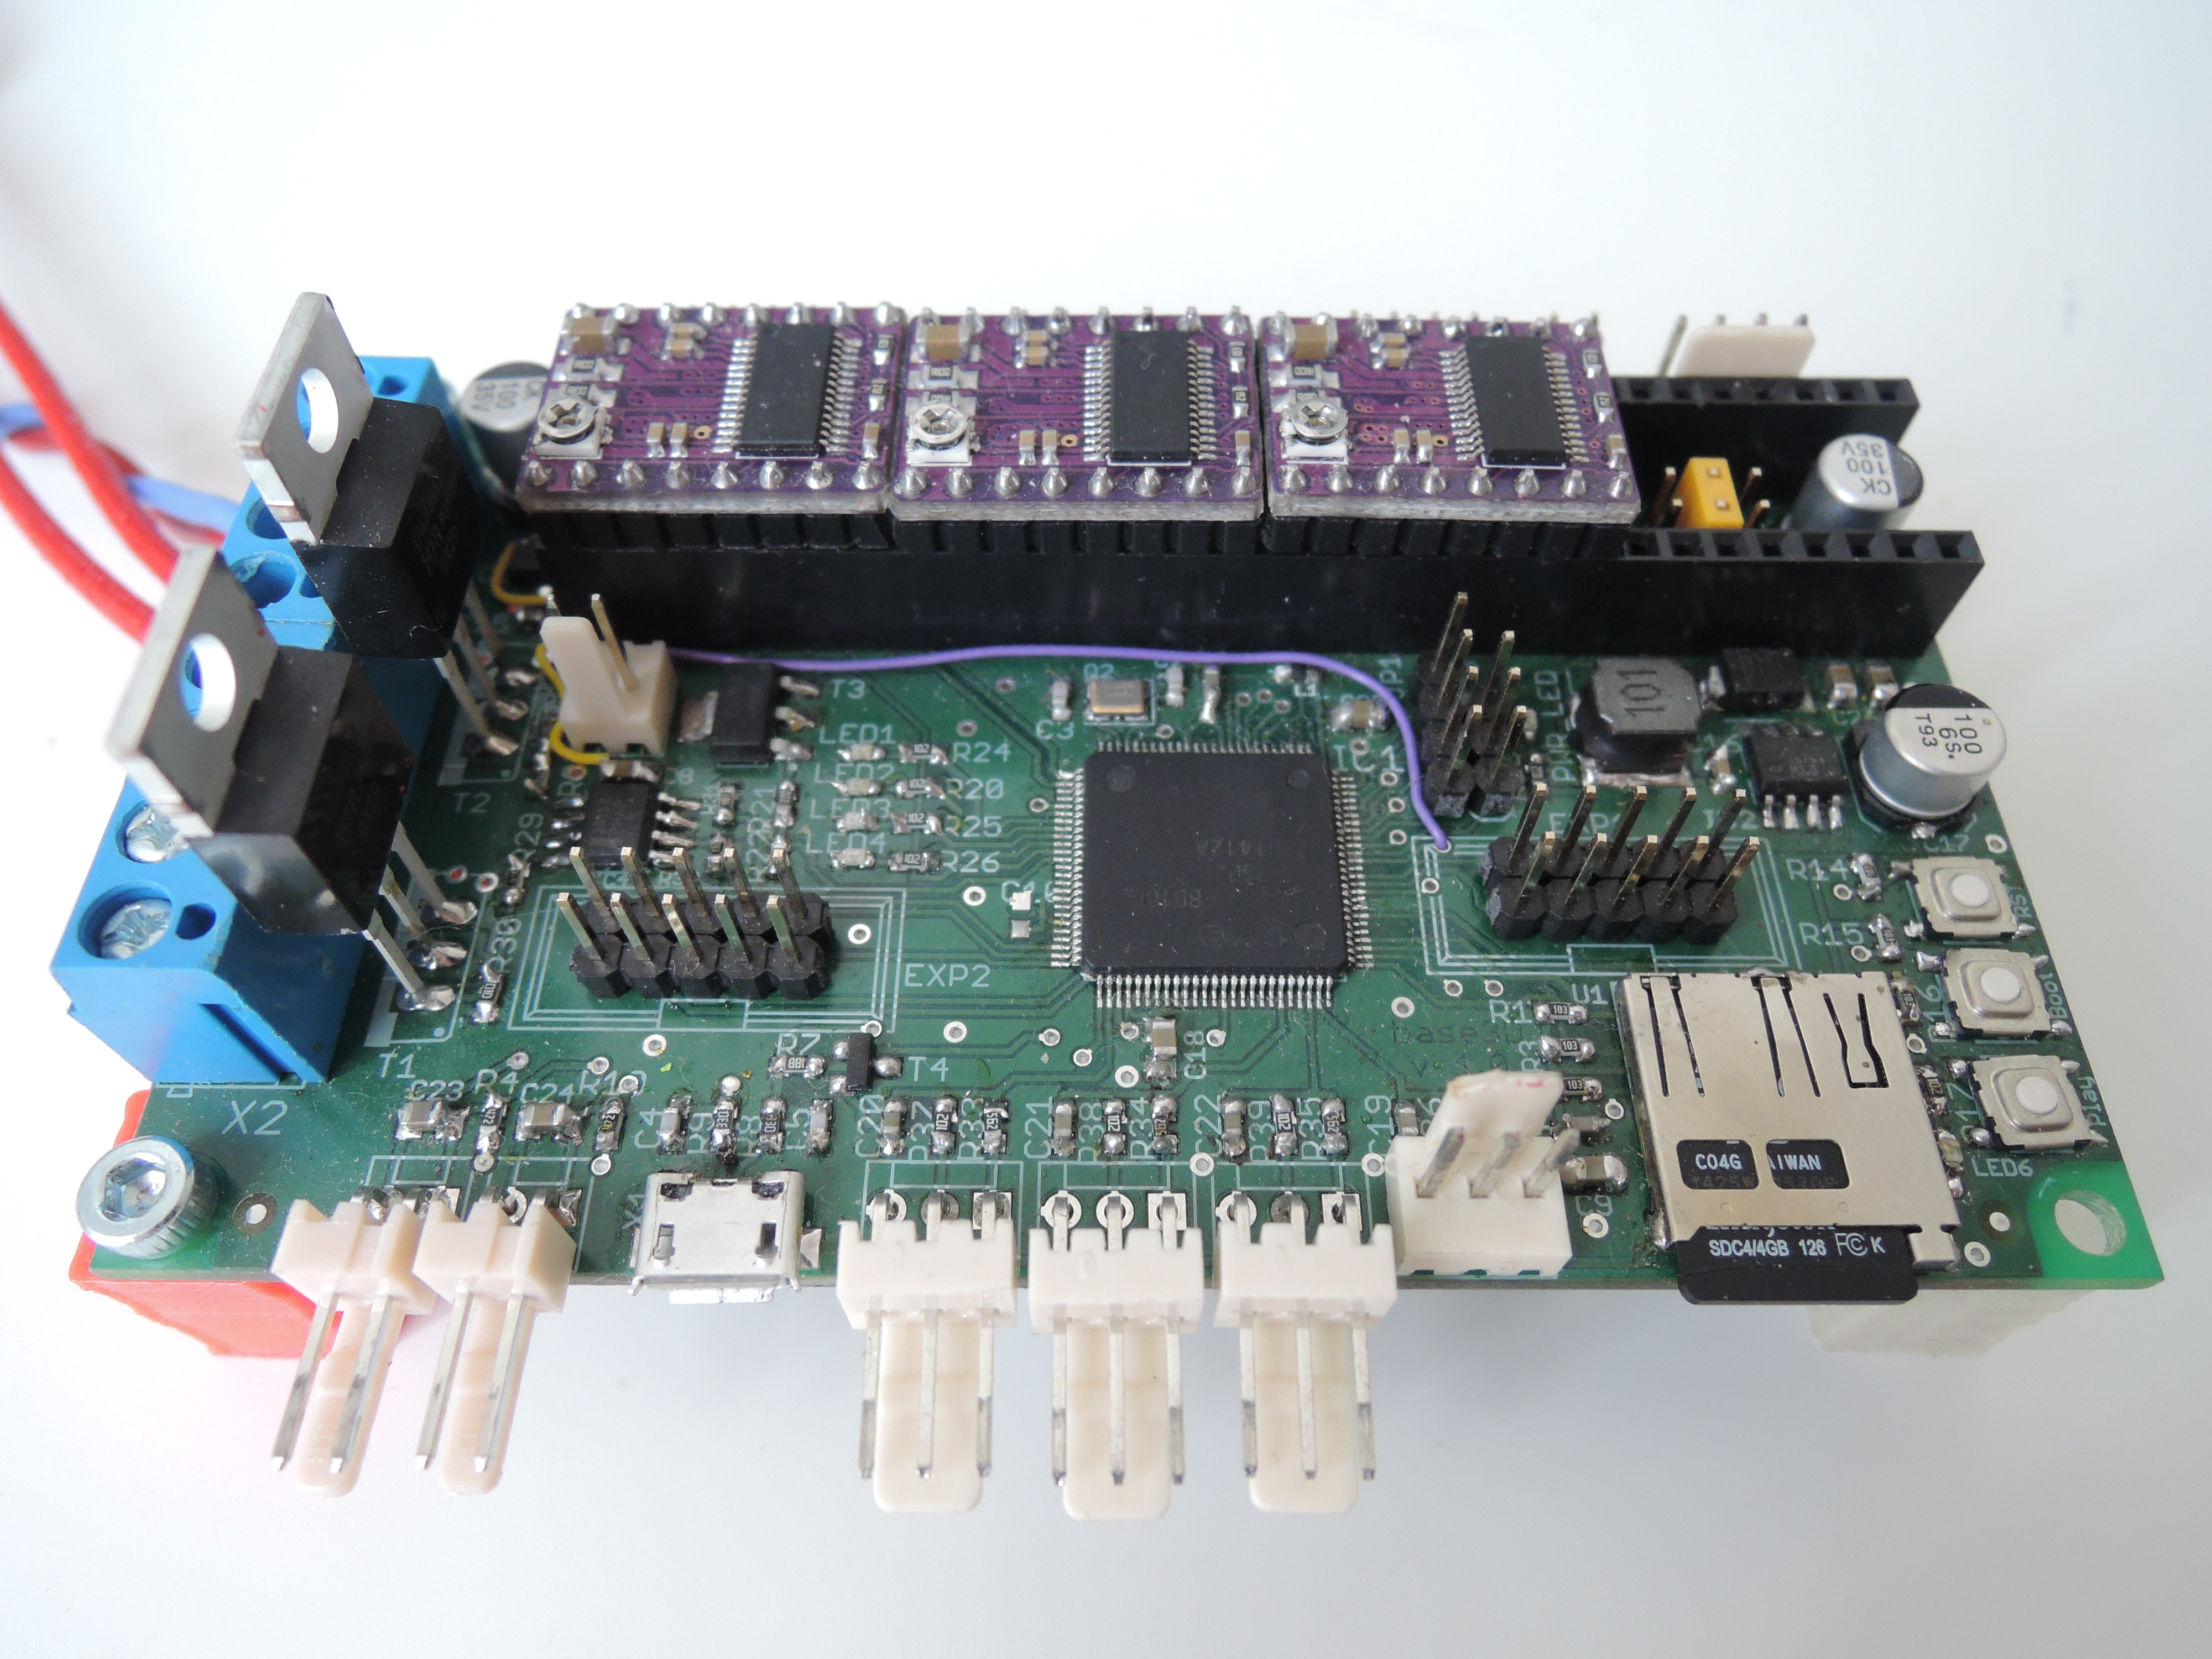
\includegraphics[width=0.8\linewidth]{obrazky/DSCN2185.JPG}%
    \caption{Osazená řídící elektronika ve verzi 1.0.}
\end{figure}




%% Vložení souboru 'text/sw' s popisem vysledků práce
\chapter{Řídící SW}

Řídící software pro osazovací automat byla nejtěžší část celého projektu. SW spojuje jednotlivé části popsané v předcházejících kapitolách do jednoho celku. 



Jeden z hlavních požadavků na řídící SW byla jeho platformová nezávislost. Tedy možnost spuštění aplikace jak na operačním systému Linux, tak i na Windows. Protože aplikace má grafické rozhraní, zúžil se výběr mnou známých programovacích jazyků na C/C++, Java, Delphi a Python. Byl vybrán  právě poslední zmiňovaný Python, jelikož má velice dobrou dokumentaci a nástroje pro tvorbu GUI jsou uživatelsky přívětivé.
Tato kombinace slibovala rychlý prototyping SW a naději na funkční SW. Pro tvorbu GUI padla volba na PyQt.

V aplikaci je kvůli centrování součástek a desek potřebné i vyhodnocování obrazu. Jako základ byla použita hojně používaná knihovna OpenCV. Ta nabízí set základních funkcí pro manipulaci s obrazem. Implementované funkce jako rozostření, hledání hran, kontur a kruhů zjednoduší úlohu rozpoznávání pozice a rotace součástek a hledání centrovacích bodů DPS.


Screenshoty z QTGUI a pár věcí ohledně PyQt







\section{Data pro osazovací automat}

Pro návrh elektronických systémů se používá software spadající do kategorie EDA – Electronic Design Automation. Je to soubor nástrojů pro tvorbu desek plošných spojů (a integrovaných obvodů). Mezi základní nástroje patří Schématické editory, simulátory obvodů, autoroutery, návrhové prostředí pro tvorbu DPS a CAM procesor. 
Příkladem EDA softwérů jsou: Altium Designer, KiCad, CadSoft Eagle.

Pro testování byl použit poslední zmiňovaný CadSoft Eagle, který je ve své základní varianě pro nekomerční účely dostupný zdarma. Uvžujme vytvořené schéma a DPS. Pro osazovací automat potřebujeme získat pozici, hodnotu, typ pouzdra a rotaci každé SMD součástky, dále potřebujeme získat pozici centrovacích značek. K tomu se částečně dají použít jendak vestavěné funkce, Eagle ale disponuje i možností použití tzv ULP (User Language Program. ) skriptů. ULP je programovací jazyk postavený na základech C a umožňuje přímé modifikování schématu, DPS a vytváření různých exportů.


Vestavěný export
Jednou z cest jak vyexportovat pozice součástek je \verb|File->Export->Partlist|


Výsledný export obsahuje všechny použité součástky a exportované pozice jsou v jednotkách mil. Pro osazovací automat je ale potřeba jen SMD součástek a centrovacích bodů. Tento export tedy není příliš vhodný, protože by potřeboval ještě následnou ruční úpravu spočívající minimálně v odmazání všech THD součástek


\begin{table}[h!]
  \caption{Ukázka exportu. }
  \begin{center}
  	\small
	  \begin{tabular}{|c|c|c|c|c|c|}
	    \hline
	    Part	& Value 	& Package 	& Library 	& Position (mil) 	& orientation	\\
	    \hline\hline

		C1 	& .1uF		& C0603		& resistor	& (2860 300)		& R180		\\
		\hline
		C2 	& 18pF		& C0603		& rcl		& (2075 1405)		& R90		\\
		\hline
	    \hline
	  \end{tabular}
  \end{center}
\end{table}

Součástí instalace Eagle je i několik již připravených ULP skriptů pro export, například Centroid\_ScreamingCircuits\_smd.ulp
Ten generuje oproti Partlistu strojově čitelnější formát a exportuje jen SMD součástky. Bohužel však chybí typ použitého pouzdra a hodnota součástky. 

\begin{verbatim}
  RefDes,Layer,LocationX,LocationY,Rotation
  C1,Top,2.860,0.300,180
  C2,Top,2.075,1.405,90
\end{verbatim}

Pro vytvoření exportu se všemi potřebnými hodnotami tak bylo potřeba napsat vlastní ULP skrip. 
Ten exportuje středy/origins součástek tak, jak byly vytvořené autorem součástky v knihovnách, dále i geomterické středy součástek. Geomterický střed funguje tak, že se iteruje nad všemi ploškami součástky a hledá se minimum a maximum v obou osách. Jejich rozdíl se vydělí dvěma a najde se skutečný střed součástky. Není to tak střed součástky základě geometrického tvaru pouzdra! Na to je třeba brát později zřetel. Důvod pro export těchto souřadnic je ten, že né všechny součástky v knihovnách se drží zažitého standardu na umisťování středícího bodu do středu pouzdra, případně do levého horního rohu.

Ukázka z ULP skriptu exportující informace o centrovacích bodech DPS

\begin{verbatim}
  printf("Part name;Package;Value;X origin;Y origin;\n");
  printf("%%fiducials\n");
  B.elements(E) if (E.populate) {

    if (E.package.name == "FIDUCIAL_1MM") 
         printf("%s;%s;%s;%.3f;%.3f;\n",
         E.name, E.package.name, E.value, u2mm(E.x), u2mm(E.y));  


  }
  printf("%%end_fiducials\n");
\end{verbatim}

Výsledný export je pak ve formátu 
\begin{verbatim}
  %data
  Part name;X center;Y center;X origin;Y origin;Rotation;Value;Package
  C1;72.644;7.620;72.644;7.620;180;.1uF;C0603
  C2;52.705;35.687;52.705;35.687;90;18pF;C0603
  %data_end
  %fiducials
  Part name;Package;Value;X origin;Y origin;
  U$3;FIDUCIAL_1MM;FIDUCIAL;7.500;3.000;
  U$4;FIDUCIAL_1MM;FIDUCIAL;7.500;57.000;
  U$6;FIDUCIAL_1MM;FIDUCIAL;92.500;3.000;
  %fiducials_end
\end{verbatim}

skript také exportuje obrázek dané DPS, který se dá po načtení do řídícího SW použít pro simulaci osazování. Celý skript je přiložen v příloze B.



%% Vložení souboru 'text/vysledky' s popisem vysledků práce
\chapter{Měření}

\section{Přesnost}
\section{Reprodukovatelnost}
Reprodukovatelnost mechanismu je po přesnosti měření 

\begin{figure}[h!]
  \centering
    \includegraphics[width=0.9\linewidth]{obrazky/repeatability.png}%
    \caption{Repeatabilita TODO.}
    \label{fig:repeatability}
\end{figure}


%% Vložení souboru 'text/zaver' se závěrem
\chapter{Závěr}

Limitace velikost soucastek, nedostatek vakua. 



SW:
Mnou stanovený požadavek na multiplatformí SW byl splněn, ale bohužel nedošlo na jeho verifikaci v praxi. Všechny testy byly prováděny pouze na operačním systému Fedora 21 (Linux).  Možná inkompatibilita hrozila v různém přístupu systémů k hardware, konkrétně k sériovému portu a dále v kompatibilitě grafického rozhraní. Pro eliminaci problémů s HW byla použita knihovna PySerial, která je dostupná ve verzích pro Windows, Linux i MacOS/X. Stejně tak použitý framework na grafické rozhraní PyQt je dostupný pro již zmíněně operační systémi.
Při spoušění programu na jiných platformách než Linux se tak nepředpokládají žádné problémy.
\\

HW:
Při návrhu a následném testování elektroniky jsem získal velice cenné zkušenosti z oblasti elektromagnetické kompatibility. První prototyp navržené elektroniky byl náchylný na elektromagnetickou susceptibilitu a z toho důvodu docházelo k výpadkům komunkace přes USB rozhraní. Po nastudování nesčetných zdrojů se povedlo v druhé revizi problém eliminovat. A to za pomocí filtrů na signálových cestách a striktním dodržení návrhových pravidel daných výrobcem mikrokontroléru.
\\

Využití:
Jak bylo naznačeno v kapitole XXX, osazovací automat může být po úpravě řídícího SW využit i pro automatickou optickou inspekci (AOI) osazených a zapájených DPS. Spojil by tak dva kroky výrobního procesu DPS do jednoho přístroje.
Realizovaná konstrukce je poměrně univerzální a mohla by najít využítí také jako manipulační robot.


%% Vložení souboru 'text/literatura' se seznamem literatury
\begin{literatura}{99}
	
\bibitem{boldis}
    BOLDIŠ, P.
    \emph{Bibliografické citace dokumentů podle ČSN ISO 690 a ČSN ISO 690-2}\/ [online].
    2001, poslední aktualizace 11.\,11.\,2004 [cit.\,17.\,2.\,2005].
    Dostupné z~URL:
    \(<\)\url{http://www.boldis.cz/citace/citace.html}\(>\).
	

\bibitem{intel}
    INTEL CORPORATION.
    \emph{Power Delivery Design Issues for Hi-Speed USB on Motherboards}\/ [online].
    2002 [cit.\,10.\,3.\,2015].
    Dostupné z~URL:
    \(<\)\url{http://www.usb.org/}\(>\).

\bibitem{vaske}
    Vaške, F.
    \emph{Design and implementation of testing device for gonio mechanisms}\/ .
    2012.

\bibitem{makerslide}
    The MakerSlide project.
    \emph{MakerSlide.}\/ [online].
    [cit.\,20.\,5.\,2015].
    Dostupné z:
    \(<\)\url{http://makerslide.com}\(>\).

\bibitem{pfeiffer}
    Pfeiffer Vacuum
    \emph{Diaphragm Pumps.}\/ [online].
    [cit.\,20.\,5.\,2015].
    Dostupné z:
    \(<\)\url{http://www.pfeiffer-vacuum.com/en/products/diaphragm-pumps/}\(>\).


\bibitem{onsemi}
    ON Semiconductor.
    \emph{Tape \& Reel Packaging Standards.} USA,
    2014, 43 stran.

\bibitem{ipcFiduc}
    IPC.
    \emph{IPC-7351 Generic Requirements for Surface Mount Design and Land Pattern Standard.}\/ [online]. 2005
    [cit.\,20.\,5.\,2015].
    Dostupné z:
    \(<\)\url{http://pcbget.ru/Files/Standarts/IPC_7351.pdf}\(>\).



\end{literatura}


%% Vložení souboru 'text/zkratky' se seznam použitých symbolů, veličin a zkratek
\begin{seznamzkratek}{KolikMista}



	\novazkratka{zkPCB}		% název
		{PCB}								% zkratka
		{Deska plošných spojů}
											% rozvinutí zkratky

	\novazkratka{zkAOI}						% název
		{AOI} % symbol
		{Automatická Optická Inspekce}					% popis

	\novazkratka{zkPnP}						% název
		{PnP} % symbol
		{Pick and Place}					% popis

	\novazkratka{zkUSB}						% název
		{USB} % symbol
		{Universal Serial Bus}					% popis
		
\end{seznamzkratek}


%% Začátek příloh
\prilohy

%% Vysázení seznamu příloh
\seznampriloh

%% Vložení souboru 'text/prilohy' s přílohami
\chapter{Některé příkazy balíčku \texttt{thesis}}\label{priloha:A}

\section{Příkazy pro sazbu veličin a jednotek}

\begin{table}[!h]
  \caption{Přehled příkazů pro matematické prostředí }
  \begin{center}
  	\small
	  \begin{tabular}{|c|c|c|c|}
	    \hline
	    Příkaz    						& Příklad 					& Zdroj příkladu  							& Význam  \\
	    \hline\hline
	    \verb|\textind{...}|	& $\beta_\textind{max}$ 	& \verb|$\beta_\textind{max}$|	& textový index \\
	    \hline
	    \verb|\konst{...}| 		& $\konst{U}_\textind{in}$ 				& \verb|$\konst{U}_\textind{in}$|		& konstantní veličina \\
	    \hline
	    \verb|\prom{...}| 		& $\prom{u}_\textind{in}$ & \verb|$\prom{u}_\textind{in}$| & proměnná veličina \\
	    \hline
	    \verb|\komplex{...}| 	& $\komplex{u}_\textind{in}$ & \verb|$\komplex{u}_\textind{in}$| & komplexní veličina \\
	    \hline
	    \verb|\vekt{...}| 		& $\vekt{y}$ 						& \verb|$\vekt{y}$| & vektor \\
	    \hline
	    \verb|\matice{...}| 	& $\matice{Z}$ 						& \verb|$\matice{Z}$| & matice \\
	    \hline
	    \verb|\jedn{...}| 		& $\jedn{kV}$ 						& \verb|$\jedn{kV}$|\quad či\ \, \verb|\jedn{kV}| & jednotka \\
	    \hline
	  \end{tabular}
  \end{center}
\end{table}



%\newpage
\section{Příkazy pro sazbu symbolů}

\begin{itemize}
  \item
    \verb|\E|, \verb|\eul| -- sazba Eulerova čísla: $\eul$,
  \item
    \verb|\J|, \verb|\jmag|, \verb|\I|, \verb|\imag| -- sazba imaginární jednotky: $\jmag$, $\imag$,
  \item
    \verb|\dif| -- sazba diferenciálu: $\dif$,
  \item
    \verb|\sinc| -- sazba funkce: $\sinc$.
  \item
    \verb|\mikro| -- sazba symbolu mikro stojatým písmem\footnote{znak pochází z~balíčku \texttt{textcomp}}: $\mikro$.

\end{itemize}
%
Všechny symboly jsou určeny pro matematický mód, vyjma \verb|\mikro|, jenž je použitelný rovněž v~textovém módu.






\chapter{Osazené DPS}\label{priloha:B}


\section{Testovací DPS C}
\begin{figure}[H]
  \centering
    \includegraphics[height=0.35\paperheight ]{obrazky/C2.jpg}%
    \caption{Testovací DPS C.}
    \label{img:DeskaC}
\end{figure}


\begin{table}[H]
  \caption{Naměřené chyby osazení pro testovací DPS C.}
  \begin{center}
  	\small
	  \begin{tabular}{|c|c|c|c|c|c|c|c|c|c|c|}
	    \hline
			& \textbf{R41}	& \textbf{R42}	& \textbf{R43}	& \textbf{R44}	& \textbf{R45}	& \textbf{R46}	& \textbf{R47}	& \textbf{R48}	& \textbf{R49}	& \textbf{R50}  \\
	    \hline
	    \textbf{x}	& 0,455&	0,364&	0,242&	0,364&	0,121&	0,091&	0,091&	0,030&	0,182&	0,06  \\
	    \hline
	    \textbf{y}	&0,212&	0,091&	0,182&	0,061&	0,364&	0,455&	0,545&	0,273&	0,212&	0,515 \\
	    \hline
			& \textbf{R51}	& \textbf{R52}	& \textbf{R53}	& \textbf{R54}	& \textbf{R55}	& \textbf{R56}	& \textbf{R57}	& \textbf{R58}	& \textbf{R59}	& \textbf{R60}  \\
	    \hline
	    \textbf{x}	&0,182&	0,212&	0,212&	0,212&	0,182&	0,000&	-0,030&	0,030&	-0,152&	0,061  \\
	    \hline
	    \textbf{y}	&0,091&	0,030&	0,303&	-0,061&	-0,030&	0,030&	-0,061&	-0,061&	-0,182&	0,030 \\
	    \hline
	    		& \textbf{R61}	& \textbf{R62}	& \textbf{R63}	& \textbf{R64}	& \textbf{R65}	& \textbf{R66}	& \textbf{R67}	& \textbf{R68}	& \textbf{R69}	& \textbf{R70}  \\
	    \hline
	    \textbf{x}	& -0,030&	0,000&	0,061&	0,000&	0,000&	-0,061&	-0,333&	-0,030&	0,030&	-0,061 \\
	    \hline
	    \textbf{y}	& 0,000&	0,030&	-0,030&	0,000&	-0,152&	0,000&	-0,091&	0,061&	0,182&	0,152 \\
	    \hline
	  \end{tabular}
  \end{center}
\end{table}




\section{Testovací DPS D}
\begin{figure}[H]
  \centering
    \includegraphics[height=0.35\paperheight ]{obrazky/D2.jpg}%
    \caption{Testovací DPS D.}
    \label{img:DeskaD}
\end{figure}


\begin{table}[H]
  \caption{Naměřené chyby osazení pro testovací DPS D.}
  \begin{center}
  	\small
	  \begin{tabular}{|c|c|c|c|c|c|c|c|c|c|c|}
	    \hline
			& \textbf{R41}	& \textbf{R42}	& \textbf{R43}	& \textbf{R44}	& \textbf{R45}	& \textbf{R46}	& \textbf{R47}	& \textbf{R48}	& \textbf{R49}	& \textbf{R50}  \\
	    \hline
	    \textbf{x}	& -0,515&	-0,485&	-1,121&	-0,818&	-1,121&	-1,424&	-1,758&	-1,576&	-1,970&	na \\
	    \hline
	    \textbf{y}	&-0,182&	-0,182&	0,212&	0,030&	0,061&	0,242&	0,576&	0,182&	0,455&	na \\
	    \hline
			& \textbf{R51}	& \textbf{R52}	& \textbf{R53}	& \textbf{R54}	& \textbf{R55}	& \textbf{R56}	& \textbf{R57}	& \textbf{R58}	& \textbf{R59}	& \textbf{R60}  \\
	    \hline
	    \textbf{x}	& -0,424&	-0,455&	-0,545&	-0,848&	-1,273&	-1,485&	-1,364&	-1,697&	-1,939&	na  \\
	    \hline
	    \textbf{y}	& 0,545&	0,545&	0,485&	0,333&	0,515&	0,242&	0,364&	0,182&	0,394&	na \\
	    \hline
	    		& \textbf{R61}	& \textbf{R62}	& \textbf{R63}	& \textbf{R64}	& \textbf{R65}	& \textbf{R66}	& \textbf{R67}	& \textbf{R68}	& \textbf{R69}	& \textbf{R70}  \\
	    \hline
	    \textbf{x}	& -0,727&	-1,030&	-1,152&	-1,394&	-1,667&	-1,606&	-1,970&	-2,091&	-2,182&	na \\
	    \hline
	    \textbf{y}	& 0,636&	0,667&	0,667&	0,788&	0,636&	0,758&	0,758&	0,636&	0,667&	na \\
	    \hline

	  \end{tabular}

  \end{center}

\end{table}







\section{Testovací DPS E}
\begin{figure}[H]
  \centering
    \includegraphics[height=0.35\paperheight ]{obrazky/E2.jpg}%
    \caption{Testovací DPS E.}
    \label{img:DeskaE}
\end{figure}



\begin{table}[H]
  \caption{Naměřené chyby osazení pro testovací DPS E.}
  \begin{center}
  	\small
	  \begin{tabular}{|c|c|c|c|c|c|c|c|c|c|c|}
	    \hline
			& \textbf{R41}	& \textbf{R42}	& \textbf{R43}	& \textbf{R44}	& \textbf{R45}	& \textbf{R46}	& \textbf{R47}	& \textbf{R48}	& \textbf{R49}	& \textbf{R50}  \\
	    \hline
	    \textbf{x}	& 0,515	& 0,515	& 0,424	& 0,394	& 0,485	& 0,515	& 0,303	& 0,273	& 0,333	& 0,333 \\
	    \hline
	    \textbf{y}	&-0,030	& 0,242	& 0,091	& 0,212	& 0,364	& 0,303	& -0,030 & 0,273 & 0,515& 0,576 \\
	    \hline
			& \textbf{R51}	& \textbf{R52}	& \textbf{R53}	& \textbf{R54}	& \textbf{R55}	& \textbf{R56}	& \textbf{R57}	& \textbf{R58}	& \textbf{R59}	& \textbf{R60}  \\
	    \hline
	    \textbf{x}	& 0,545	& 0,333	& 0,515	& 0,182	& 0,242	& 0,333	& 0,333	& 0,333	& 0,091	& 0,242  \\
	    \hline
	    \textbf{y}	& 0,333	& 0,273	& 0,152	& 0,061	& -0,030& -0,182& -0,242& -0,152& -0,364& -0,242 \\
	    \hline
	    		& \textbf{R61}	& \textbf{R62}	& \textbf{R63}	& \textbf{R64}	& \textbf{R65}	& \textbf{R66}	& \textbf{R67}	& \textbf{R68}	& \textbf{R69}	& \textbf{R70}  \\
	    \hline
	    \textbf{x}	& 0,000	& 0,152	& 0,212	& 0,333	& 0,121	& 0,273	& 0,242	& 0,030	& 0,061	& -0,333 \\
	    \hline
	    \textbf{y}	& 0,000	& -0,030& 0,121	& -0,273& 0,000	& -0,061& 0,030	& 0,000	& 0,000	& 0,212 \\
	    \hline

	  \end{tabular}

  \end{center}

\end{table}


\chapter{Obsah přiloženého CD}\label{priloha:C}

Nezapomeňte uvést, co čtenář najde na přiloženém médiu.
Je vhodné okomentovat obsah každého adresáře, specifikovat, který soubor obsahuje důležitá nastavení, který soubor je určen ke spuštění atd.
Také je dobře napsat, v~jaké verzi software byl kód testován (např.\ Matlab 2010b).


%% Konec dokumentu
\end{document}
